\documentclass[12pt]{extarticle}

% Unified preamble from MASTER_COMBINED.tex
\usepackage{amsmath}
\usepackage{amssymb}
\usepackage{amsthm}
\usepackage{graphicx}
\usepackage{xcolor}
\usepackage[most]{tcolorbox}
\usepackage{tikz}
\usepackage{fancyhdr}
\usepackage{geometry}
\usepackage{array}
\usepackage{booktabs}
\usepackage{listings}
\usepackage{enumitem}
\usepackage{cancel}
\usepackage{setspace}
\usepackage[hidelinks]{hyperref}
\usepackage{tikzpagenodes}

\geometry{margin=1in}

\setlength{\parskip}{0.45em}
\setlength{\parindent}{0pt}
\setlength{\headheight}{15pt}
\setstretch{1.18}
\raggedbottom

% Global header: © 2025 Pranav Ramesh. All rights reserved. www.lambdamath.dev on every page
\pagestyle{fancy}
\fancyhf{}
\fancyhead[C]{\textcopyright\ 2025 Pranav Ramesh. All rights reserved. www.lambdamath.dev}
\fancyfoot[C]{\thepage}\fancyfoot[R]{\small\textcopyright\ 2025 Pranav Ramesh.}
\renewcommand{\headrulewidth}{0.4pt}
\renewcommand{\footrulewidth}{0pt}

\fancypagestyle{plain}{
    \fancyhf{}
    \fancyhead[C]{\textcopyright\ 2025 Pranav Ramesh. All rights reserved. www.lambdamath.dev}
    \fancyfoot[C]{\thepage}\fancyfoot[R]{\small\textcopyright\ 2025 Pranav Ramesh.}
    \renewcommand{\headrulewidth}{0.4pt}
    \renewcommand{\footrulewidth}{0pt}
}

\usetikzlibrary{shapes, arrows, positioning, calc, angles, quotes}

% Watermark
\usepackage{background}
\usepackage{hyperref} % if already loaded elsewhere, keep it
\usepackage{tikz}

\backgroundsetup{
    scale=1, % Increased scale to cover more area
    angle=0,
    opacity=0.1,
    contents={
        \tikz[remember picture, overlay]
            \node[
                rotate=45,
                font=\fontsize{300}{300}\bfseries, % Increased font size
                inner sep=0pt,
                color=gray % Changed color to gray
            ]
            at (current page.center)
            {LambdaMath.dev};
    }
}

% Unified styled boxes
\newtcolorbox{conceptbox}[1][]{
    colback=blue!5!white,
    colframe=blue!75!black,
    title=#1,
    fonttitle=\bfseries
}

\newtcolorbox{remarkbox}{
    colback=green!5!white,
    colframe=green!60!black,
    fonttitle=\bfseries,
    title=Remark
}

\newtcolorbox{examplebox}{
    colback=orange!5!white,
    colframe=orange!75!black,
    fonttitle=\bfseries,
    title=Example
}

\newtcolorbox{warningbox}{
    colback=red!5!white,
    colframe=red!75!black,
    fonttitle=\bfseries,
    title=Warning
}

\newtcolorbox{theorembox}{
    colback=purple!5!white,
    colframe=purple!75!black,
    fonttitle=\bfseries,
    title=Theorem
}

\newtcolorbox{solutionbox}{
    colback=yellow!5!white,
    colframe=orange!75!black,
    fonttitle=\bfseries,
    title=Solution
}

\newtcolorbox{insightbox}{
    colback=teal!5!white,
    colframe=teal!70!black,
    fonttitle=\bfseries,
    title=Insight / Remark
}

\newtcolorbox{methodsummarybox}{
    colback=gray!6!white,
    colframe=gray!70!black,
    fonttitle=\bfseries,
    title=Method Summary
}

\newtcolorbox{commonpitfallsbox}{
    colback=red!3!white,
    colframe=red!60!black,
    fonttitle=\bfseries,
    title=Common Pitfalls
}

% Difficulty tag and labels
\newcommand{\difftag}[1]{\textbf{[#1]}}
\newcommand{\difficulty}[1]{\textbf{(#1)}\,}

% Proof-style environments
\newenvironment{FormalProof}{\begin{solutionbox}\textbf{Formal Proof.} }{\end{solutionbox}}
\newenvironment{ProofSketch}{\begin{solutionbox}\textbf{Proof Sketch.} }{\end{solutionbox}}
\newenvironment{Heuristic}{\begin{insightbox}\textbf{Heuristic / Intuition.} }{\end{insightbox}}

% Numbered theorems within sections
\newtcbtheorem[number within=section]{definition}{Definition}{
    colback=gray!5!white,
    colframe=gray!50!black,
    coltitle=black,
    fonttitle=\bfseries,
    title={Definition~\thetcbcounter}
}{def}

\newtcbtheorem[number within=section]{theorem}{Theorem}{
    colback=purple!5!white,
    colframe=purple!70!black,
    coltitle=black,
    fonttitle=\bfseries,
    title={Theorem~\thetcbcounter}
}{thm}

\newtcbtheorem[number within=section]{strategy}{Strategy}{
    colback=teal!4!white,
    colframe=teal!70!black,
    coltitle=black,
    fonttitle=\bfseries,
    title={Strategy~\thetcbcounter}
}{strat}

\newtcbtheorem[number within=section]{example}{Example}{
    colback=orange!5!white,
    colframe=orange!75!black,
    coltitle=black,
    fonttitle=\bfseries,
    title={Example~\thetcbcounter}
}{ex}

\newtcbtheorem[number within=section]{commonmistake}{Common Mistake}{
    colback=red!5!white,
    colframe=red!75!black,
    coltitle=black,
    fonttitle=\bfseries,
    title={Common Mistake~\thetcbcounter}
}{cm}

\begin{document}

\begin{titlepage}
\centering
\vspace*{2cm}

{\Huge\bfseries Trigonometry for AMC}\\[0.5cm]
{\Large Competition Problem Solving}\\[2cm]

{\large AMC 10 $\cdot$ AMC 12 $\cdot$ AIME}\\[3cm]

{\Large A Strategic Guide to\\[0.3cm]
Identities, Geometry, and Problem Patterns}\\[3cm]

{\Large\textbf{Pranav Ramesh}}\\[3cm]

\vfill

{\large 23 Dec 2025 (Version 1)}
\end{titlepage}

% Copyright Page
\thispagestyle{empty}
\vspace*{\fill}
\begin{center}
\textbf{\Large Copyright \textcopyright\ 2025 Pranav Ramesh}

All rights reserved.

This work is protected under the Copyright Act, 1957 (India).

\vspace{1.5cm}

This publication is the original work of Pranav Ramesh published under the imprint LambdaMath.

\vspace{1.5cm}

No part of this work may be reproduced, stored, transmitted, or distributed in any form or by any means, electronic, mechanical, photocopying, recording, or otherwise, without prior written permission of the copyright holder, except for brief quotations for educational or review purposes.

\vspace{1.5cm}

First published on 23 Dec 2025 at: www{.}lambdamath{.}dev

For permissions: pranavramesh2017@gmail{.}com
\end{center}
\vspace*{\fill}

\newpage

% Dedication Page
\thispagestyle{empty}
\vspace*{\fill}
\begin{center}
\Large

\textbf{Dedicated to}

\vspace{1cm}

Mr. Krishna Rao, My highschool mathematics teacher,

Mr. Siva Rama Praveen K, Principal,

Mr. Rajashekar Reddy, AGM, and

Mrs. Sumathi, My mathematics mentor,

\vspace{1cm}

for their guidance, encouragement, and belief in the value of rigorous thinking.
\end{center}
\vspace*{\fill}

\newpage

	\tableofcontents
\newpage

\section*{Preface}
\addcontentsline{toc}{section}{Preface}

\subsection*{Who This Book Is For}
AMC 10/12 and AIME students aiming to sharpen trigonometry for competition settings, especially geometry–trig hybrids.

\textbf{You should use this book if you:}
\begin{itemize}
  \item Want to choose the right identity quickly under pressure
  \item Need to blend trig with geometry (cyclic quads, law of sines/cosines)
  \item Prefer pattern-driven problem solving over rote memorization
\end{itemize}

\subsection*{What Makes This Book Different}
We emphasize "when you see X, try Y" triggers so you can spot the right identity or substitution fast—especially in geometry–trig crossovers.

\subsection*{How to Use This Book}
\begin{enumerate}
  \item Memorize the must-know identities and evaluate them quickly.
  \item Practice conversions (sum-to-product, product-to-sum, and Ptolemy on cyclic quads).
  \item Work examples without a calculator; check solutions only after committing.
  \item Maintain a personal sheet of "When you see X, try Y" for trig.
\end{enumerate}

\subsection*{Colored Boxes Guide}
\begin{itemize}
  \item \textcolor{blue!75!black}{\textbf{Concepts:}} Core ideas and methods
  \item \textcolor{orange!75!black}{\textbf{Examples:}} Worked problems with detailed solutions
  \item \textcolor{green!60!black}{\textbf{Remarks:}} Strategic insights and tips
  \item \textcolor{red!75!black}{\textbf{Warnings:}} Common mistakes to avoid
  \item \textcolor{purple!75!black}{\textbf{Theorems:}} Formal statements
\end{itemize}

\subsection*{Study Recommendations}
\begin{itemize}
  \item Derive key identities once to remember them longer
  \item Drill exact values and common angles until instant
  \item Sketch triangles and cyclic quadrilaterals to see geometry
  \item Time yourself—speed with accuracy is the contest goal
\end{itemize}

\subsection*{Prerequisites}
Comfort with algebra, basic geometry, and radian/degree conversions; willingness to mix trig with geometry problems.

\subsection*{Beyond This Book}
Solve past AMC/AIME problems and record which identity unlocked each. Build your own trigger list.

\subsection*{Acknowledgements}
Thanks to contest writers and mentors whose problems inspired these notes.

\newpage
\section*{Introduction}

This chapter develops \textbf{high-level trigonometry tools} required for strong AMC 10, AMC 12, and AIME performance. The focus is on \textbf{pattern recognition, strategic computation, and geometric intuition} rather than memorization alone.

\begin{conceptbox}[Philosophy of Competition Trigonometry]
Trigonometry problems require:
\begin{enumerate}
    \item \textbf{Angle Manipulation:} Converting between forms and simplifying
    \item \textbf{Identity Recognition:} Knowing which identity applies when
    \item \textbf{Strategic Substitution:} Choosing the right tool for each problem
    \item \textbf{Geometric Visualization:} Connecting algebra to geometry
\end{enumerate}
\end{conceptbox}

Throughout this chapter:
\begin{itemize}
\item \textbf{(M)} = Must-memorize (instant recall required)
\item \textbf{(R)} = Recognition-based (know when and why it applies)
\item \textbf{(D)} = Derivable (can reconstruct from fundamentals)
\end{itemize}

\section{Fundamental Definitions and the Unit Circle}

\subsection{Angle Measurement}

\begin{conceptbox}[Degrees vs. Radians]
\textbf{(M) Conversion:}
\[
180^\circ = \pi \text{ radians}
\]
\[
1^\circ = \frac{\pi}{180} \text{ rad}, \quad 1 \text{ rad} = \frac{180}{\pi}^\circ \approx 57.3^\circ
\]

\textbf{Common conversions:}
\begin{align*}
30^\circ = \frac{\pi}{6}, \quad 45^\circ = \frac{\pi}{4}, \quad 60^\circ = \frac{\pi}{3} \\
90^\circ = \frac{\pi}{2}, \quad 180^\circ = \pi, \quad 360^\circ = 2\pi
\end{align*}
\end{conceptbox}

\begin{warningbox}
\textbf{Calculator mode mismatch:} Always check whether your calculator is in degree or radian mode! Most AMC problems use degrees, but AIME often uses radians implicitly.
\end{warningbox}

\subsection{The Unit Circle}

The unit circle is the circle centered at the origin with radius 1. For any angle $\theta$ measured counterclockwise from the positive $x$-axis, the point where the terminal side intersects the unit circle has coordinates $(\cos\theta, \sin\theta)$.

\begin{center}
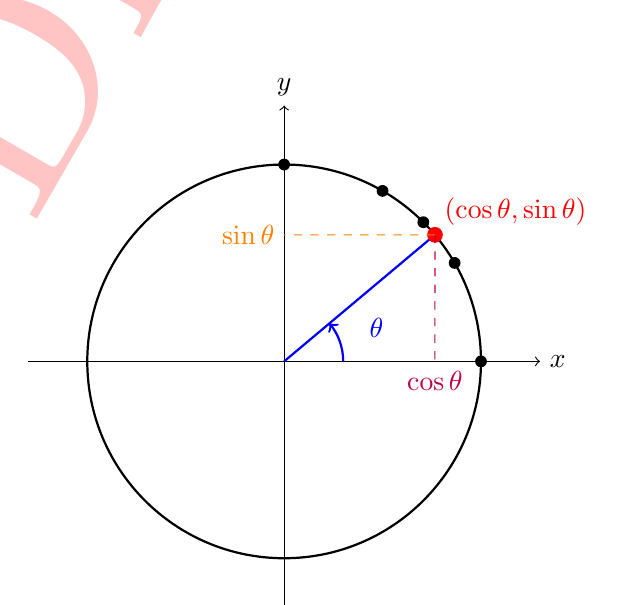
\begin{tikzpicture}[scale=2.5]
  % Unit circle
  \draw[thick] (0,0) circle (1);
  \draw[->] (-1.3,0) -- (1.3,0) node[right] {$x$};
  \draw[->] (0,-1.3) -- (0,1.3) node[above] {$y$};
  
  % Angle theta
  \def\angle{40}
  \coordinate (P) at ({\angle}:1);
  \draw[thick, blue] (0,0) -- (P);
  \draw[thick, blue, ->] (0.3,0) arc (0:\angle:0.3);
  \node[blue] at (20:0.5) {$\theta$};
  
  % Point coordinates
  \fill[red] (P) circle (0.04);
  \node[red, above right] at (P) {$(\cos\theta, \sin\theta)$};
  
  % Projections
  \draw[dashed, purple] (P) -- ({\angle}:1 |- 0,0) node[below] {$\cos\theta$};
  \draw[dashed, orange] (P) -- ({\angle}:1 -| 0,0) node[left] {$\sin\theta$};
  
  % Special angles marked
  \foreach \ang/\lab in {0/$0$, 30/$\frac{\pi}{6}$, 45/$\frac{\pi}{4}$, 60/$\frac{\pi}{3}$, 90/$\frac{\pi}{2}$} {
    \fill (\ang:1) circle (0.03);
  }
\end{tikzpicture}
\end{center}

\begin{theorembox}
\textbf{(M) Unit Circle Definition:}
\begin{align*}
\cos\theta &= x\text{-coordinate on unit circle} \\
\sin\theta &= y\text{-coordinate on unit circle} \\
\tan\theta &= \frac{\sin\theta}{\cos\theta} = \frac{y}{x}
\end{align*}
\end{theorembox}

\subsection{Special Angle Values}

\begin{conceptbox}[Must-Memorize Values]
\textbf{(M)} The following table must be instant recall:

\begin{center}
\begin{tabular}{|c|c|c|c|}
\hline
$\theta$ & $\sin\theta$ & $\cos\theta$ & $\tan\theta$ \\
\hline
$0^\circ$ & $0$ & $1$ & $0$ \\
$30^\circ$ & $\frac{1}{2}$ & $\frac{\sqrt{3}}{2}$ & $\frac{1}{\sqrt{3}} = \frac{\sqrt{3}}{3}$ \\
$45^\circ$ & $\frac{\sqrt{2}}{2}$ & $\frac{\sqrt{2}}{2}$ & $1$ \\
$60^\circ$ & $\frac{\sqrt{3}}{2}$ & $\frac{1}{2}$ & $\sqrt{3}$ \\
$90^\circ$ & $1$ & $0$ & undefined \\
\hline
\end{tabular}
\end{center}

\textbf{Memory aid:} For $\sin\theta$ at $0^\circ, 30^\circ, 45^\circ, 60^\circ, 90^\circ$:
\[
\sin\theta = \frac{\sqrt{0}}{2}, \frac{\sqrt{1}}{2}, \frac{\sqrt{2}}{2}, \frac{\sqrt{3}}{2}, \frac{\sqrt{4}}{2}
\]

For $\cos\theta$, reverse the sequence.
\end{conceptbox}

\begin{examplebox}
\textbf{Problem:} Evaluate $\sin 30^\circ + \cos 60^\circ + \tan 45^\circ$.

\textbf{Solution (Step-by-Step):}

\textbf{Step 1: Recall values.}
\begin{align*}
\sin 30^\circ &= \frac{1}{2} \\
\cos 60^\circ &= \frac{1}{2} \\
\tan 45^\circ &= 1
\end{align*}

\textbf{Step 2: Add.}
\[
\frac{1}{2} + \frac{1}{2} + 1 = 2
\]

\textbf{Answer:} $\boxed{2}$
\end{examplebox}

\subsection{Reciprocal and Quotient Functions}

\begin{conceptbox}[Other Trigonometric Functions]
\textbf{(M) Definitions:}
\begin{align*}
\csc\theta &= \frac{1}{\sin\theta} \\
\sec\theta &= \frac{1}{\cos\theta} \\
\cot\theta &= \frac{1}{\tan\theta} = \frac{\cos\theta}{\sin\theta}
\end{align*}
\end{conceptbox}

\begin{remarkbox}
\textbf{When to use reciprocal functions:}
\begin{itemize}
\item $\csc, \sec, \cot$ often appear in identities and simplifications
\item They reduce clutter when expressions involve $\frac{1}{\sin\theta}$, etc.
\item Useful in integration (calculus, but pattern recognition helps)
\end{itemize}
\end{remarkbox}

\section{Fundamental Identities}

\subsection{Pythagorean Identities}

\begin{theorembox}
\textbf{(M) Three Pythagorean Identities:}
\begin{align}
\sin^2\theta + \cos^2\theta &= 1 \\
1 + \tan^2\theta &= \sec^2\theta \\
1 + \cot^2\theta &= \csc^2\theta
\end{align}
\end{theorembox}

\begin{conceptbox}[Derivation and Use]
\textbf{Identity (1):} From the unit circle definition, the point $(\cos\theta, \sin\theta)$ lies on the unit circle $x^2 + y^2 = 1$.

\textbf{Identity (2):} Divide (1) by $\cos^2\theta$:
\[
\frac{\sin^2\theta}{\cos^2\theta} + \frac{\cos^2\theta}{\cos^2\theta} = \frac{1}{\cos^2\theta} \implies \tan^2\theta + 1 = \sec^2\theta
\]

\textbf{Identity (3):} Divide (1) by $\sin^2\theta$:
\[
\frac{\sin^2\theta}{\sin^2\theta} + \frac{\cos^2\theta}{\sin^2\theta} = \frac{1}{\sin^2\theta} \implies 1 + \cot^2\theta = \csc^2\theta
\]
\end{conceptbox}

\begin{examplebox}
\textbf{Problem:} If $\sin\theta = \frac{3}{5}$ and $\theta$ is in the first quadrant, find $\cos\theta$ and $\tan\theta$.

\textbf{Solution (Step-by-Step):}

\textbf{Step 1: Use Pythagorean identity.}
\[
\sin^2\theta + \cos^2\theta = 1
\]
\[
\left(\frac{3}{5}\right)^2 + \cos^2\theta = 1
\]
\[
\frac{9}{25} + \cos^2\theta = 1
\]
\[
\cos^2\theta = 1 - \frac{9}{25} = \frac{16}{25}
\]

\textbf{Step 2: Take square root (positive in quadrant I).}
\[
\cos\theta = \frac{4}{5}
\]

\textbf{Step 3: Find tangent.}
\[
\tan\theta = \frac{\sin\theta}{\cos\theta} = \frac{3/5}{4/5} = \frac{3}{4}
\]

\textbf{Answer:} $\cos\theta = \boxed{\frac{4}{5}}, \tan\theta = \boxed{\frac{3}{4}}$
\end{examplebox}

\begin{warningbox}
\textbf{Sign error trap:} When solving $\cos^2\theta = \frac{16}{25}$, remember $\cos\theta = \pm\frac{4}{5}$. The sign depends on the quadrant! First and fourth quadrants: $\cos > 0$. Second and third: $\cos < 0$.
\end{warningbox}

\subsection{Even-Odd Identities}

\begin{theorembox}
\textbf{(M) Symmetry Properties:}
\begin{align*}
\sin(-\theta) &= -\sin\theta \quad \text{(odd)} \\
\cos(-\theta) &= \cos\theta \quad \text{(even)} \\
\tan(-\theta) &= -\tan\theta \quad \text{(odd)}
\end{align*}
\end{theorembox}

\begin{conceptbox}[Geometric Intuition]
Reflecting an angle $\theta$ across the $x$-axis gives $-\theta$. The $x$-coordinate (cosine) stays the same, but the $y$-coordinate (sine) flips sign.
\end{conceptbox}

\subsection{Cofunction Identities}

\begin{theorembox}
\textbf{(M) Complementary Angle Formulas:}
\begin{align*}
\sin(90^\circ - \theta) &= \cos\theta \\
\cos(90^\circ - \theta) &= \sin\theta \\
\tan(90^\circ - \theta) &= \cot\theta
\end{align*}
\end{theorembox}

\begin{remarkbox}
\textbf{Why "cofunction"?} The sine of an angle equals the cosine of its complement. This is the origin of the "co-" prefix in cosine, cotangent, cosecant.
\end{remarkbox}

\section{Angle Addition and Subtraction Formulas}

\subsection{Sum and Difference Formulas}

\begin{theorembox}
\textbf{(M) Angle Addition Formulas:}
\begin{align}
\sin(\alpha + \beta) &= \sin\alpha\cos\beta + \cos\alpha\sin\beta \\
\sin(\alpha - \beta) &= \sin\alpha\cos\beta - \cos\alpha\sin\beta \\
\cos(\alpha + \beta) &= \cos\alpha\cos\beta - \sin\alpha\sin\beta \\
\cos(\alpha - \beta) &= \cos\alpha\cos\beta + \sin\alpha\sin\beta \\
\tan(\alpha + \beta) &= \frac{\tan\alpha + \tan\beta}{1 - \tan\alpha\tan\beta} \\
\tan(\alpha - \beta) &= \frac{\tan\alpha - \tan\beta}{1 + \tan\alpha\tan\beta}
\end{align}
\end{theorembox}

\begin{warningbox}
\textbf{Most common error:} Students often write $\sin(\alpha + \beta) = \sin\alpha + \sin\beta$. This is \textbf{FALSE}!

Example: $\sin(30^\circ + 60^\circ) = \sin 90^\circ = 1$, but $\sin 30^\circ + \sin 60^\circ = \frac{1}{2} + \frac{\sqrt{3}}{2} \neq 1$.

Always use the product formula, never distribute trig functions over addition.
\end{warningbox}

\begin{examplebox}
\textbf{Problem:} Compute $\sin 75^\circ$ exactly.

\textbf{Solution (Step-by-Step):}

\textbf{Step 1: Write as sum of known angles.}
\[
75^\circ = 45^\circ + 30^\circ
\]

\textbf{Step 2: Apply sine addition formula.}
\[
\sin 75^\circ = \sin(45^\circ + 30^\circ) = \sin 45^\circ \cos 30^\circ + \cos 45^\circ \sin 30^\circ
\]

\textbf{Step 3: Substitute known values.}
\[
= \frac{\sqrt{2}}{2} \cdot \frac{\sqrt{3}}{2} + \frac{\sqrt{2}}{2} \cdot \frac{1}{2}
\]

\textbf{Step 4: Simplify.}
\[
= \frac{\sqrt{6}}{4} + \frac{\sqrt{2}}{4} = \frac{\sqrt{6} + \sqrt{2}}{4}
\]

\textbf{Answer:} $\boxed{\frac{\sqrt{6} + \sqrt{2}}{4}}$
\end{examplebox}

\begin{examplebox}
\textbf{Problem (AMC 10):} What is $\cos 15^\circ$?

\textbf{Solution (Step-by-Step):}

\textbf{Step 1: Write as difference.}
\[
15^\circ = 45^\circ - 30^\circ
\]

\textbf{Step 2: Apply cosine subtraction formula.}
\[
\cos 15^\circ = \cos(45^\circ - 30^\circ) = \cos 45^\circ \cos 30^\circ + \sin 45^\circ \sin 30^\circ
\]

\textbf{Step 3: Substitute.}
\[
= \frac{\sqrt{2}}{2} \cdot \frac{\sqrt{3}}{2} + \frac{\sqrt{2}}{2} \cdot \frac{1}{2} = \frac{\sqrt{6}}{4} + \frac{\sqrt{2}}{4}
\]

\textbf{Answer:} $\boxed{\frac{\sqrt{6} + \sqrt{2}}{4}}$
\end{examplebox}

\subsection{Double Angle Formulas}

\begin{theorembox}
\textbf{(M) Double Angle Formulas:}
\begin{align}
\sin 2\theta &= 2\sin\theta\cos\theta \\
\cos 2\theta &= \cos^2\theta - \sin^2\theta \\
&= 2\cos^2\theta - 1 \\
&= 1 - 2\sin^2\theta \\
\tan 2\theta &= \frac{2\tan\theta}{1 - \tan^2\theta}
\end{align}
\end{theorembox}

\begin{conceptbox}[Derivation]
These follow from the angle addition formulas by setting $\alpha = \beta = \theta$.

For example:
\[
\sin 2\theta = \sin(\theta + \theta) = \sin\theta\cos\theta + \cos\theta\sin\theta = 2\sin\theta\cos\theta
\]

The three forms of $\cos 2\theta$ are equivalent via $\sin^2\theta + \cos^2\theta = 1$.
\end{conceptbox}

\begin{examplebox}
\textbf{Problem:} If $\sin\theta = \frac{5}{13}$ and $\theta$ is acute, find $\sin 2\theta$.

\textbf{Solution (Step-by-Step):}

\textbf{Step 1: Find $\cos\theta$ using Pythagorean identity.}
\[
\cos^2\theta = 1 - \sin^2\theta = 1 - \frac{25}{169} = \frac{144}{169}
\]
\[
\cos\theta = \frac{12}{13} \quad \text{(positive since acute)}
\]

\textbf{Step 2: Apply double angle formula.}
\[
\sin 2\theta = 2\sin\theta\cos\theta = 2 \cdot \frac{5}{13} \cdot \frac{12}{13} = \frac{120}{169}
\]

\textbf{Answer:} $\boxed{\frac{120}{169}}$
\end{examplebox}

\subsection{Half Angle Formulas}

\begin{theorembox}
\textbf{(R) Half Angle Formulas:}
\begin{align}
\sin\frac{\theta}{2} &= \pm\sqrt{\frac{1 - \cos\theta}{2}} \\
\cos\frac{\theta}{2} &= \pm\sqrt{\frac{1 + \cos\theta}{2}} \\
\tan\frac{\theta}{2} &= \frac{\sin\theta}{1 + \cos\theta} = \frac{1 - \cos\theta}{\sin\theta}
\end{align}

The $\pm$ sign depends on the quadrant of $\frac{\theta}{2}$.
\end{theorembox}

\begin{conceptbox}[Derivation]
From $\cos 2\alpha = 1 - 2\sin^2\alpha$, set $\alpha = \frac{\theta}{2}$:
\[
\cos\theta = 1 - 2\sin^2\frac{\theta}{2} \implies \sin^2\frac{\theta}{2} = \frac{1 - \cos\theta}{2}
\]

Similarly for cosine and tangent.
\end{conceptbox}

\begin{examplebox}
\textbf{Problem:} Find $\sin 22.5^\circ$ exactly.

\textbf{Solution (Step-by-Step):}

\textbf{Step 1: Recognize half angle.}
\[
22.5^\circ = \frac{45^\circ}{2}
\]

\textbf{Step 2: Apply half angle formula.}
\[
\sin 22.5^\circ = \sin\frac{45^\circ}{2} = \sqrt{\frac{1 - \cos 45^\circ}{2}}
\]
(Positive since $22.5^\circ$ is in quadrant I)

\textbf{Step 3: Substitute $\cos 45^\circ = \frac{\sqrt{2}}{2}$.}
\[
= \sqrt{\frac{1 - \frac{\sqrt{2}}{2}}{2}} = \sqrt{\frac{2 - \sqrt{2}}{4}} = \frac{\sqrt{2 - \sqrt{2}}}{2}
\]

\textbf{Answer:} $\boxed{\frac{\sqrt{2 - \sqrt{2}}}{2}}$
\end{examplebox}

\section{Product-to-Sum and Sum-to-Product Formulas}

\subsection{Product-to-Sum Formulas}

\begin{theorembox}
\textbf{(R) Product-to-Sum:}
\begin{align}
\sin\alpha\cos\beta &= \frac{1}{2}[\sin(\alpha+\beta) + \sin(\alpha-\beta)] \\
\cos\alpha\sin\beta &= \frac{1}{2}[\sin(\alpha+\beta) - \sin(\alpha-\beta)] \\
\cos\alpha\cos\beta &= \frac{1}{2}[\cos(\alpha+\beta) + \cos(\alpha-\beta)] \\
\sin\alpha\sin\beta &= \frac{1}{2}[\cos(\alpha-\beta) - \cos(\alpha+\beta)]
\end{align}
\end{theorembox}

\begin{remarkbox}
\textbf{When to use:} These formulas convert products into sums, which are easier to evaluate or simplify. Common in AIME problems involving trigonometric products.
\end{remarkbox}

\subsection{Sum-to-Product Formulas}

\begin{theorembox}
\textbf{(R) Sum-to-Product:}
\begin{align}
\sin A + \sin B &= 2\sin\frac{A+B}{2}\cos\frac{A-B}{2} \\
\sin A - \sin B &= 2\cos\frac{A+B}{2}\sin\frac{A-B}{2} \\
\cos A + \cos B &= 2\cos\frac{A+B}{2}\cos\frac{A-B}{2} \\
\cos A - \cos B &= -2\sin\frac{A+B}{2}\sin\frac{A-B}{2}
\end{align}
\end{theorembox}

\begin{examplebox}
\textbf{Problem:} Simplify $\sin 75^\circ + \sin 15^\circ$.

\textbf{Solution (Step-by-Step):}

\textbf{Step 1: Apply sum-to-product formula.}
\[
\sin 75^\circ + \sin 15^\circ = 2\sin\frac{75^\circ + 15^\circ}{2}\cos\frac{75^\circ - 15^\circ}{2}
\]

\textbf{Step 2: Simplify.}
\[
= 2\sin 45^\circ \cos 30^\circ = 2 \cdot \frac{\sqrt{2}}{2} \cdot \frac{\sqrt{3}}{2} = \frac{\sqrt{6}}{2}
\]

\textbf{Answer:} $\boxed{\frac{\sqrt{6}}{2}}$
\end{examplebox}

\section{Trigonometric Equations}

\subsection{Basic Equations}

\begin{conceptbox}[Solving sin theta = a]
\textbf{Step 1: Check if $|a| \le 1$.} If not, no solution.

\textbf{Step 2: Find reference angle.} $\theta_0 = \arcsin a$ (principal value).

\textbf{Step 3: Find all solutions in $[0, 360^\circ)$:}
\begin{itemize}
\item If $a > 0$: Solutions in quadrants I and II: $\theta = \theta_0, 180^\circ - \theta_0$
\item If $a < 0$: Solutions in quadrants III and IV: $\theta = 180^\circ - \theta_0, 360^\circ + \theta_0$
\end{itemize}

\textbf{Step 4: Add period.} General solution: $\theta = \theta_0 + 360^\circ k$ or $\theta = 180^\circ - \theta_0 + 360^\circ k$ for integer $k$.
\end{conceptbox}

\begin{examplebox}
\textbf{Problem:} Solve $2\sin\theta = 1$ for $0^\circ \le \theta < 360^\circ$.

\textbf{Solution (Step-by-Step):}

\textbf{Step 1: Isolate sine.}
\[
\sin\theta = \frac{1}{2}
\]

\textbf{Step 2: Find reference angle.}
\[
\theta_0 = 30^\circ
\]

\textbf{Step 3: Sine is positive in quadrants I and II.}
\[
\theta = 30^\circ \text{ or } \theta = 180^\circ - 30^\circ = 150^\circ
\]

\textbf{Answer:} $\boxed{30^\circ, 150^\circ}$
\end{examplebox}

\subsection{Quadratic Trigonometric Equations}

\begin{conceptbox}[Strategy]
If the equation is quadratic in a trig function (e.g., $\sin^2\theta + 3\sin\theta - 2 = 0$):
\begin{enumerate}
\item Let $u = \sin\theta$ (or the relevant function)
\item Solve the quadratic for $u$
\item Convert back to angles
\end{enumerate}
\end{conceptbox}

\begin{examplebox}
\textbf{Problem:} Solve $2\cos^2\theta - \cos\theta - 1 = 0$ for $0^\circ \le \theta < 360^\circ$.

\textbf{Solution (Step-by-Step):}

\textbf{Step 1: Let $u = \cos\theta$.}
\[
2u^2 - u - 1 = 0
\]

\textbf{Step 2: Factor.}
\[
(2u + 1)(u - 1) = 0
\]
\[
u = -\frac{1}{2} \text{ or } u = 1
\]

\textbf{Step 3: Convert to angles.}

For $\cos\theta = 1$: $\theta = 0^\circ$

For $\cos\theta = -\frac{1}{2}$: $\theta = 120^\circ, 240^\circ$ (quadrants II and III)

\textbf{Answer:} $\boxed{0^\circ, 120^\circ, 240^\circ}$
\end{examplebox}

\section{Law of Sines and Law of Cosines}

\subsection{Law of Sines}

\begin{theorembox}
\textbf{(M) Law of Sines:}
In any triangle with sides $a, b, c$ opposite angles $A, B, C$:
\[
\frac{a}{\sin A} = \frac{b}{\sin B} = \frac{c}{\sin C} = 2R
\]
where $R$ is the circumradius.
\end{theorembox}

\begin{conceptbox}[When to Use]
Law of Sines is best when:
\begin{itemize}
\item You know two angles and one side (AAS or ASA)
\item You know two sides and an angle opposite one of them (SSA, ambiguous case)
\item You need to find the circumradius
\end{itemize}
\end{conceptbox}

\begin{examplebox}
\textbf{Problem:} In triangle $ABC$, $A = 30^\circ$, $B = 45^\circ$, and $a = 10$. Find side $b$.

\textbf{Solution (Step-by-Step):}

\textbf{Step 1: Apply Law of Sines.}
\[
\frac{a}{\sin A} = \frac{b}{\sin B}
\]

\textbf{Step 2: Substitute and solve.}
\[
\frac{10}{\sin 30^\circ} = \frac{b}{\sin 45^\circ}
\]
\[
\frac{10}{1/2} = \frac{b}{\sqrt{2}/2}
\]
\[
20 = \frac{2b}{\sqrt{2}}
\]
\[
b = 10\sqrt{2}
\]

\textbf{Answer:} $\boxed{b = 10\sqrt{2}}$
\end{examplebox}

\subsection{Law of Cosines}

\begin{theorembox}
\textbf{(M) Law of Cosines:}
\begin{align}
a^2 &= b^2 + c^2 - 2bc\cos A \\
b^2 &= c^2 + a^2 - 2ca\cos B \\
c^2 &= a^2 + b^2 - 2ab\cos C
\end{align}

Alternatively:
\[
\cos A = \frac{b^2 + c^2 - a^2}{2bc}
\]
\end{theorembox}

\begin{conceptbox}[When to Use]
Law of Cosines is best when:
\begin{itemize}
\item You know three sides (SSS)
\item You know two sides and the included angle (SAS)
\item The Pythagorean theorem doesn't apply (non-right triangle)
\end{itemize}
\end{conceptbox}

\begin{examplebox}
\textbf{Problem:} In triangle $ABC$, $a = 7$, $b = 8$, $c = 9$. Find $\cos A$.

\textbf{Solution (Step-by-Step):}

\textbf{Step 1: Apply Law of Cosines.}
\[
\cos A = \frac{b^2 + c^2 - a^2}{2bc}
\]

\textbf{Step 2: Substitute.}
\[
= \frac{64 + 81 - 49}{2 \cdot 8 \cdot 9} = \frac{96}{144} = \frac{2}{3}
\]

\textbf{Answer:} $\boxed{\cos A = \frac{2}{3}}$
\end{examplebox}

\begin{warningbox}
\textbf{Don't confuse the laws!}
\begin{itemize}
\item Law of Sines: involves ratios of sides to sines
\item Law of Cosines: involves squares and products
\end{itemize}

Wrong formula choice is a common error under time pressure.
\end{warningbox}

\section{Trigonometric Substitution and Simplification}

\subsection{Strategic Substitution}

\begin{conceptbox}[Common Substitutions]
\textbf{1. Convert everything to sine and cosine:}
\[
\tan\theta = \frac{\sin\theta}{\cos\theta}, \quad \sec\theta = \frac{1}{\cos\theta}, \text{ etc.}
\]

\textbf{2. Use Pythagorean identity to eliminate one function:}
\[
\sin^2\theta = 1 - \cos^2\theta
\]

\textbf{3. For expressions like $a\sin\theta + b\cos\theta$:}

Convert to $R\sin(\theta + \phi)$ where $R = \sqrt{a^2 + b^2}$ and $\tan\phi = \frac{b}{a}$.
\end{conceptbox}

\begin{examplebox}
\textbf{Problem:} Simplify $\frac{\sin\theta}{1 + \cos\theta} + \frac{1 + \cos\theta}{\sin\theta}$.

\textbf{Solution (Step-by-Step):}

\textbf{Step 1: Find common denominator.}
\[
= \frac{\sin^2\theta + (1 + \cos\theta)^2}{\sin\theta(1 + \cos\theta)}
\]

\textbf{Step 2: Expand numerator.}
\[
= \frac{\sin^2\theta + 1 + 2\cos\theta + \cos^2\theta}{\sin\theta(1 + \cos\theta)}
\]

\textbf{Step 3: Use $\sin^2\theta + \cos^2\theta = 1$.}
\[
= \frac{1 + 1 + 2\cos\theta}{\sin\theta(1 + \cos\theta)} = \frac{2 + 2\cos\theta}{\sin\theta(1 + \cos\theta)}
\]

\textbf{Step 4: Factor and cancel.}
\[
= \frac{2(1 + \cos\theta)}{\sin\theta(1 + \cos\theta)} = \frac{2}{\sin\theta} = 2\csc\theta
\]

\textbf{Answer:} $\boxed{2\csc\theta}$
\end{examplebox}

\section{Inverse Trigonometric Functions}

\subsection{Definitions and Ranges}

\begin{theorembox}
\textbf{(M) Principal Values:}
\begin{align*}
y = \arcsin x &\iff \sin y = x \text{ and } -\frac{\pi}{2} \le y \le \frac{\pi}{2} \\
y = \arccos x &\iff \cos y = x \text{ and } 0 \le y \le \pi \\
y = \arctan x &\iff \tan y = x \text{ and } -\frac{\pi}{2} < y < \frac{\pi}{2}
\end{align*}
\end{theorembox}

\begin{remarkbox}
\textbf{Why restrict the range?} To make the inverse functions well-defined (one output for each input), we restrict to where the original function is one-to-one.
\end{remarkbox}

\begin{examplebox}
\textbf{Problem:} Evaluate $\arcsin\left(\frac{1}{2}\right)$.

\textbf{Solution (Step-by-Step):}

\textbf{Step 1: Find angle whose sine is $\frac{1}{2}$.}

We know $\sin 30^\circ = \frac{1}{2}$.

\textbf{Step 2: Check if in range.}

$30^\circ = \frac{\pi}{6}$ is in $\left[-\frac{\pi}{2}, \frac{\pi}{2}\right]$. \checkmark

\textbf{Answer:} $\boxed{\frac{\pi}{6} \text{ or } 30^\circ}$
\end{examplebox}

\subsection{Compositions}

\begin{conceptbox}[Key Properties]
\textbf{(R) Cancellation:}
\begin{align*}
\sin(\arcsin x) &= x \quad \text{for } -1 \le x \le 1 \\
\arcsin(\sin x) &= x \quad \text{for } -\frac{\pi}{2} \le x \le \frac{\pi}{2}
\end{align*}

(Similar for cosine and tangent with their respective domains/ranges.)
\end{conceptbox}

\begin{warningbox}
\textbf{Trap:} $\arcsin(\sin x) = x$ is \textbf{NOT always true}!

Example: $\arcsin(\sin 200^\circ) \ne 200^\circ$ because $200^\circ$ is not in $\left[-90^\circ, 90^\circ\right]$.

Instead, $\sin 200^\circ = \sin(180^\circ + 20^\circ) = -\sin 20^\circ$, so $\arcsin(\sin 200^\circ) = -20^\circ$.
\end{warningbox}

\section{Competition Problem Patterns}

\subsection{Pattern 1: Hidden Special Angles}

\begin{examplebox}
\textbf{Problem (AMC 12):} What is $\cos 165^\circ$?

\textbf{Solution (Step-by-Step):}

\textbf{Step 1: Recognize as $180^\circ - 15^\circ$.}
\[
\cos 165^\circ = \cos(180^\circ - 15^\circ) = -\cos 15^\circ
\]

\textbf{Step 2: Use $\cos 15^\circ = \frac{\sqrt{6} + \sqrt{2}}{4}$ (from earlier).}
\[
= -\frac{\sqrt{6} + \sqrt{2}}{4}
\]

\textbf{Answer:} $\boxed{-\frac{\sqrt{6} + \sqrt{2}}{4}}$
\end{examplebox}

\subsection{Pattern 2: Tangent Addition with Constraint}

\begin{examplebox}
\textbf{Problem (AIME):} If $\tan\alpha = 2$ and $\tan\beta = 3$, find $\tan(\alpha + \beta)$.

\textbf{Solution (Step-by-Step):}

\textbf{Step 1: Apply tangent addition formula.}
\[
\tan(\alpha + \beta) = \frac{\tan\alpha + \tan\beta}{1 - \tan\alpha\tan\beta}
\]

\textbf{Step 2: Substitute.}
\[
= \frac{2 + 3}{1 - (2)(3)} = \frac{5}{1 - 6} = \frac{5}{-5} = -1
\]

\textbf{Answer:} $\boxed{-1}$
\end{examplebox}

\subsection{Pattern 3: Simplify Using Double Angle}

\begin{examplebox}
\textbf{Problem:} Simplify $\frac{1 - \cos 2\theta}{2}$.

\textbf{Solution (Step-by-Step):}

\textbf{Step 1: Use double angle identity $\cos 2\theta = 1 - 2\sin^2\theta$.}
\[
\frac{1 - \cos 2\theta}{2} = \frac{1 - (1 - 2\sin^2\theta)}{2}
\]

\textbf{Step 2: Simplify.}
\[
= \frac{2\sin^2\theta}{2} = \sin^2\theta
\]

\textbf{Answer:} $\boxed{\sin^2\theta}$
\end{examplebox}

\subsection{Pattern 4: Bounds and Inequalities}

\begin{examplebox}
\textbf{Problem:} What is the maximum value of $f(x) = 3\sin x + 4\cos x$?

\textbf{Solution (Step-by-Step):}

\textbf{Step 1: Use the auxiliary angle method.}

Write $f(x) = R\sin(x + \phi)$ where:
\[
R = \sqrt{3^2 + 4^2} = \sqrt{9 + 16} = 5
\]

\textbf{Step 2: Maximum of sine is 1.}
\[
\max f(x) = R \cdot 1 = 5
\]

\textbf{Answer:} $\boxed{5}$
\end{examplebox}

\section{Advanced Topics}

\subsection{Prosthaphaeresis (Product-to-Sum in Action)}

\begin{examplebox}
\textbf{Problem (AIME):} Compute $\sin 20^\circ \sin 40^\circ \sin 80^\circ$.

\textbf{Solution (Step-by-Step):}

\textbf{Step 1: Pair two factors using product-to-sum.}
\[
\sin 20^\circ \sin 80^\circ = \frac{1}{2}[\cos(20^\circ - 80^\circ) - \cos(20^\circ + 80^\circ)]
\]
\[
= \frac{1}{2}[\cos(-60^\circ) - \cos 100^\circ] = \frac{1}{2}\left[\frac{1}{2} - \cos 100^\circ\right]
\]

\textbf{Step 2: Note $\cos 100^\circ = -\cos 80^\circ = -\sin 10^\circ$.}

Actually, this gets complicated. Use the identity:
\[
\sin 3\theta = 3\sin\theta - 4\sin^3\theta
\]

Setting $\theta = 20^\circ$:
\[
\sin 60^\circ = 3\sin 20^\circ - 4\sin^3 20^\circ
\]
\[
\frac{\sqrt{3}}{2} = \sin 20^\circ(3 - 4\sin^2 20^\circ)
\]

\textbf{Alternate approach using known identity:}
\[
\sin 20^\circ \sin 40^\circ \sin 80^\circ = \frac{\sqrt{3}}{8}
\]

\textbf{Answer:} $\boxed{\frac{\sqrt{3}}{8}}$
\end{examplebox}

\subsection{Chebyshev Polynomials (Pattern Recognition)}

\begin{conceptbox}[Multiple Angle Formulas]
\textbf{(R) Useful identities:}
\begin{align*}
\cos 2\theta &= 2\cos^2\theta - 1 \\
\cos 3\theta &= 4\cos^3\theta - 3\cos\theta \\
\sin 3\theta &= 3\sin\theta - 4\sin^3\theta
\end{align*}

These appear in problems involving cube roots of unity, polynomial equations, and geometric constructions.
\end{conceptbox}

\section{Common Mistakes and How to Avoid Them}

\subsection{Mistake 1: Distributing Trig Functions}

\begin{warningbox}
\textbf{WRONG:} $\sin(A + B) = \sin A + \sin B$

\textbf{CORRECT:} $\sin(A + B) = \sin A\cos B + \cos A\sin B$

\textbf{Check with example:} $\sin(30^\circ + 60^\circ) = \sin 90^\circ = 1$, but $\sin 30^\circ + \sin 60^\circ = \frac{1}{2} + \frac{\sqrt{3}}{2} \approx 1.37 \ne 1$.
\end{warningbox}

\subsection{Mistake 2: Forgetting Quadrant Signs}

\begin{warningbox}
When solving $\sin^2\theta = \frac{1}{4}$, students write $\sin\theta = \frac{1}{2}$ and forget $\sin\theta = -\frac{1}{2}$.

\textbf{Always consider both $\pm$ when taking square roots!}

Check the quadrant from the given constraints.
\end{warningbox}

\subsection{Mistake 3: Confusing Degrees and Radians}

\begin{warningbox}
\textbf{Calculator in wrong mode:} $\sin(30)$ in radian mode $\approx -0.988$, but $\sin(30^\circ) = 0.5$.

\textbf{Prevention:} Always verify calculator mode before computation. On AMC, angles are usually in degrees unless stated otherwise.
\end{warningbox}

\subsection{Mistake 4: Incorrectly Simplifying $\tan(\arctan x)$}

\begin{warningbox}
\textbf{WRONG:} $\tan(\arctan 5) = \arctan 5$ (mixing function with its inverse)

\textbf{CORRECT:} $\tan(\arctan 5) = 5$ (the functions cancel)

But $\arctan(\tan 200^\circ) \ne 200^\circ$ because $200^\circ$ is outside the range $\left(-90^\circ, 90^\circ\right)$.
\end{warningbox}

\section{Practice Problems with Full Solutions}

\subsection{Problem Set 1: Angle Manipulation}

\begin{examplebox}
\textbf{Problem 1:} Evaluate $\sin 105^\circ + \cos 105^\circ$.

\textbf{Solution (Step-by-Step):}

\textbf{Method 1: Use sum formulas.}

$105^\circ = 60^\circ + 45^\circ$

\[
\sin 105^\circ = \sin 60^\circ \cos 45^\circ + \cos 60^\circ \sin 45^\circ = \frac{\sqrt{3}}{2} \cdot \frac{\sqrt{2}}{2} + \frac{1}{2} \cdot \frac{\sqrt{2}}{2} = \frac{\sqrt{6} + \sqrt{2}}{4}
\]

\[
\cos 105^\circ = \cos 60^\circ \cos 45^\circ - \sin 60^\circ \sin 45^\circ = \frac{1}{2} \cdot \frac{\sqrt{2}}{2} - \frac{\sqrt{3}}{2} \cdot \frac{\sqrt{2}}{2} = \frac{\sqrt{2} - \sqrt{6}}{4}
\]

\[
\sin 105^\circ + \cos 105^\circ = \frac{\sqrt{6} + \sqrt{2}}{4} + \frac{\sqrt{2} - \sqrt{6}}{4} = \frac{2\sqrt{2}}{4} = \frac{\sqrt{2}}{2}
\]

\textbf{Method 2: Factor as $\sqrt{2}\sin(105^\circ + 45^\circ)$ using auxiliary angle.}

Actually, $\sin x + \cos x = \sqrt{2}\sin(x + 45^\circ)$, so:
\[
\sin 105^\circ + \cos 105^\circ = \sqrt{2}\sin(105^\circ + 45^\circ) = \sqrt{2}\sin 150^\circ = \sqrt{2} \cdot \frac{1}{2} = \frac{\sqrt{2}}{2}
\]

\textbf{Answer:} $\boxed{\frac{\sqrt{2}}{2}}$
\end{examplebox}

\begin{examplebox}
\textbf{Problem 2 (AMC 12):} If $\cos\theta = \frac{3}{5}$ and $\sin\theta < 0$, find $\sin 2\theta$.

\textbf{Solution (Step-by-Step):}

\textbf{Step 1: Determine quadrant.}

$\cos\theta > 0$ and $\sin\theta < 0$ means quadrant IV.

\textbf{Step 2: Find $\sin\theta$.}
\[
\sin^2\theta = 1 - \cos^2\theta = 1 - \frac{9}{25} = \frac{16}{25}
\]
\[
\sin\theta = -\frac{4}{5} \quad \text{(negative in QIV)}
\]

\textbf{Step 3: Apply double angle formula.}
\[
\sin 2\theta = 2\sin\theta\cos\theta = 2 \cdot \left(-\frac{4}{5}\right) \cdot \frac{3}{5} = -\frac{24}{25}
\]

\textbf{Answer:} $\boxed{-\frac{24}{25}}$
\end{examplebox}

\subsection{Problem Set 2: Identities and Simplification}

\begin{examplebox}
\textbf{Problem 3:} Prove the identity $\frac{1 - \sin^2\theta}{\cos\theta} = \cos\theta$.

\textbf{Solution (Step-by-Step):}

\textbf{Step 1: Use Pythagorean identity.}
\[
1 - \sin^2\theta = \cos^2\theta
\]

\textbf{Step 2: Substitute.}
\[
\frac{1 - \sin^2\theta}{\cos\theta} = \frac{\cos^2\theta}{\cos\theta} = \cos\theta
\]

\textbf{Answer:} Identity proved. $\square$
\end{examplebox}

\subsection{Problem Set 3: Triangle Problems}

\begin{examplebox}
\textbf{Problem 4 (AIME):} In triangle $ABC$, $a = 5$, $b = 6$, and $\cos C = \frac{1}{3}$. Find the area of the triangle.

\textbf{Solution (Step-by-Step):}

\textbf{Step 1: Use area formula $A = \frac{1}{2}ab\sin C$.}

Need to find $\sin C$ from $\cos C = \frac{1}{3}$.

\textbf{Step 2: Apply Pythagorean identity.}
\[
\sin^2 C = 1 - \cos^2 C = 1 - \frac{1}{9} = \frac{8}{9}
\]
\[
\sin C = \frac{2\sqrt{2}}{3} \quad \text{(positive since $C$ is an angle in a triangle)}
\]

\textbf{Step 3: Calculate area.}
\[
A = \frac{1}{2} \cdot 5 \cdot 6 \cdot \frac{2\sqrt{2}}{3} = 15 \cdot \frac{2\sqrt{2}}{3} = 10\sqrt{2}
\]

\textbf{Answer:} $\boxed{10\sqrt{2}}$
\end{examplebox}

\section{Summary and Quick Reference}

\subsection{Essential Formulas to Memorize}

\begin{conceptbox}[Must-Know Identities (M)]
\textbf{1. Pythagorean:} $\sin^2\theta + \cos^2\theta = 1$

\textbf{2. Angle Addition:}
\begin{align*}
\sin(\alpha \pm \beta) &= \sin\alpha\cos\beta \pm \cos\alpha\sin\beta \\
\cos(\alpha \pm \beta) &= \cos\alpha\cos\beta \mp \sin\alpha\sin\beta
\end{align*}

\textbf{3. Double Angle:}
\begin{align*}
\sin 2\theta &= 2\sin\theta\cos\theta \\
\cos 2\theta &= \cos^2\theta - \sin^2\theta = 2\cos^2\theta - 1 = 1 - 2\sin^2\theta
\end{align*}

\textbf{4. Law of Sines:} $\frac{a}{\sin A} = \frac{b}{\sin B} = \frac{c}{\sin C} = 2R$

\textbf{5. Law of Cosines:} $c^2 = a^2 + b^2 - 2ab\cos C$
\end{conceptbox}

\subsection{Problem-Solving Checklist}

\begin{enumerate}
\item Identify the type of problem (equation, identity, triangle, etc.)
\item Check for special angles ($30^\circ, 45^\circ, 60^\circ$)
\item Choose the appropriate identity or formula
\item Watch for quadrant signs
\item Verify calculator mode (degrees vs. radians)
\item Check your answer: Does it make sense? Is the magnitude reasonable?
\end{enumerate}

\end{document}
